%
% LO, Li-yu 
%

\documentclass[a4paper,12pt]{article}

\usepackage{graphicx}
\usepackage[english]{babel}
\usepackage[]{amsmath}
\usepackage{amsfonts}
\usepackage{mathtools}
\usepackage{amssymb}
\usepackage[a4paper, portrait, margin=0.8in]{geometry}
\usepackage{hyperref}
\usepackage{algorithm,algpseudocode}
\usepackage{indentfirst}
\usepackage{soul}
\usepackage{color}
% \usepackage{subfigure}
\usepackage{titling}
% \usepackage{subcaption}
\usepackage{subfig}
\usepackage[labelfont=bf, justification=justified]{caption}
% \usepackage[demo]{graphicx}% Remove demo option in real document


\setlength{\droptitle}{-4em}   % This is your set screw

\begin{document}
%
   \title{\textbf{COMP5212 Machine Learning} \\  
   Homework 3}
   
   \author{LO, Li-yu \\ 20997405 \\ e-mail: lloac@connect.hkust.hk}
   \date{\today}
   \maketitle

\section*{Problem 1 - Proximal Gradient Descent}
\subsection*{(a)}
With the objective function being:
\begin{align*}
   \min_{\textbf{w}} \|X\textbf{w} - y\|^2_2 + \lambda \|\textbf{w}\|_1, \\ 
   X \in R^{n \times d}, \textbf{w} \in R^d, y \in R^n. 
\end{align*}
With the L1-norm, the whole thing could be further written as:
\begin{align*}
   &\min_{\textbf{w}} \|X\textbf{w} - y\|^2_2 + \lambda \|\textbf{w}\|_1, \\ 
   =&\min_{\textbf{w}} \|X\textbf{w} - y\|^2_2 + \lambda \sum_{i=1}^{d} |\textbf{w}_i|. 
\end{align*}
From the term $\sum_{i=1}^{d} \|\textbf{w}_i\|$, it could be seen that it is not a
continuous function, and it is particularly not differentiable when $\textbf{w}_i = 0$. 
Therefore, the objective function is non-differentiable, leading the inapplicability of 
gradient descent algorithm.

\subsection*{(b)}
Here we derive the closed-form solution $\textbf{w}_{t+1}$ based on the given $\textbf{w}_t$,
$\nabla g(\textbf{w}_t)$, $\eta$, and $\lambda$.
Also not that 
\begin{align}
   \label{func:proximal_mapping}
   \textbf{w}_{t+1} = arg \min_{\textbf{w}} (\hat{g}(\textbf{w}_t) + \lambda \|\textbf{w}\|_1).
\end{align}
And with:
\begin{align}
   \label{func:quadratic}
   \hat{g}(\textbf{w}_t) := g(\textbf{w}_t) + \nabla g(\textbf{w}_t)^T(\textbf{w} - \textbf{w}_t) 
   + \frac{\eta}{2} \|\textbf{w} - \textbf{w}_t\|^2_2
   % = arg \min_{\textbf{w}} (\hat{g}(\textbf{w}_t) + \lambda \|\textbf{w}\|_1).
\end{align}
First, we rewrite $\hat{g}(\textbf{w}_t)$:
\begin{align*}
   &\hat{g}(\textbf{w}_t) = g(\textbf{w}_t) + \nabla g(\textbf{w}_t)^T(\textbf{w} - \textbf{w}_t) + \frac{\eta}{2} \|\textbf{w} - \textbf{w}_t\|^2_2
   \\ &= \frac{\eta}{2} [\frac{2}{\eta} g(\textbf{w}_t) + \frac{2}{\eta}\nabla g(\textbf{w}_t)^T(\textbf{w} - \textbf{w}_t)+\|\textbf{w} - \textbf{w}_t\|^2_2]
   \\ &= \frac{\eta}{2} [\frac{2}{\eta} g(\textbf{w}_t) + \frac{2}{\eta}\nabla g(\textbf{w}_t)^T(\textbf{w} - \textbf{w}_t)+\|\textbf{w} - \textbf{w}_t\|^2_2 
   + \| \frac{1}{\eta}\nabla g(\textbf{w}_t) \|^2_2 - \|\frac{1}{\eta}\nabla g(\textbf{w}_t)\|^2_2]
   \\ &= \frac{\eta}{2}[\frac{2}{\eta} g(\textbf{w}_t) - \|\frac{1}{\eta}\nabla g(\textbf{w}_t)\|^2_2 + \| (\textbf{w} - \textbf{w}_t) + \frac{1}{\eta}\nabla g(\textbf{w}_t)  \|^2_2]
   \\ &= g(\textbf{w}_t) - \frac{\eta}{2}\|\frac{1}{\eta}\nabla g(\textbf{w}_t)\|^2_2 + \frac{\eta}{2}\| (\textbf{w} - \textbf{w}_t) + \frac{1}{\eta}\nabla g(\textbf{w}_t)  \|^2_2
\end{align*}
As $\textbf{w}_t$ is not a variable, eqn. \ref{func:proximal_mapping} is equivalent to:
\begin{align}
   \hat{g}(\textbf{w}_t) = arg \min_{\textbf{w}} (\frac{\eta}{2}\| (\textbf{w} - \textbf{w}_t) + \frac{1}{\eta}\nabla g(\textbf{w}_t)  \|^2_2 + \lambda \|\textbf{w}\|_1).
\end{align}
We also let $\textbf{w}' = \textbf{w}_t - \frac{1}{\eta}\nabla g(\textbf{w}_t)$, then we have:
\begin{align}
   \label{func:proximal_mapping2}
   \nonumber \textbf{w}_{t+1} &= arg \min_{\textbf{w}} (\frac{\eta}{2}\| \textbf{w} - \textbf{w}' \|^2_2 + \lambda \|\textbf{w}\|_1) \\ 
                    &= arg \min_{\textbf{w}} (\frac{\eta}{2} \sum_{i=1}^{d} (\textbf{w}_i - \textbf{w}_i')^2  + \lambda \sum_{i=1}^{d} \|\textbf{w}_i\|).
\end{align}
Secondly, as we know the optimality condition for a non-differentiable objective function could be derived with subgradients.
We say $w^{*}$ is a minimizer i.f.f.:
\begin{align}
   \label{func:cond}
   0 \in \{ g | g \in R^d, subgradient \; of \;  \textbf{w}^*\}
\end{align}
From eqn. \ref{func:proximal_mapping2}, we could treat the problem element-wise, and with cond. \ref{func:cond}, 
in our case, the following condition should be true:
\begin{align}
   0 \in \{ \eta (\textbf{w}_i - \textbf{w}_i')+\lambda \partial |\textbf{w}_i|  \}
\end{align}
Finally, we derive the minimizer. As 
\begin{align}
   \partial |\textbf{w}_i|
   =\begin{cases}
      1, & if \; \textbf{w} > 0.\\
      [-1,1], & if \; \textbf{w} = 0.\\
      -1, & if \; \textbf{w} < 0.\\
    \end{cases}
\end{align}
And we let:
\begin{align}
   0&=\eta (\textbf{w}_i - \textbf{w}_i')+\lambda \partial |\textbf{w}_i| \\
   \rightarrow \textbf{w}_i &= \textbf{w}_i' - \frac{1}{\eta}\lambda \partial |\textbf{w}_i|
\end{align}
Therefore, we have:
\begin{align}
   \textbf{w}_i = 
   \begin{cases}
      \textbf{w}_i' - \frac{1}{\eta} \lambda, & if \; \textbf{w}_i' > \frac{1}{\eta}\lambda.\\
      0, & if \; |\textbf{w}_i'| \leq \frac{1}{\eta}\lambda.\\
      \textbf{w}_i' + \frac{1}{\eta} \lambda, & if \; \textbf{w}_i' < -\frac{1}{\eta}\lambda.\\
    \end{cases}
\end{align}
The above is equivalent to: % $\textbf{w}' = \textbf{w}_t - \frac{1}{\eta}\nabla g(\textbf{w}_t)$
\begin{align}
   \textbf{w}_i = 
   \begin{cases}
      [\textbf{w}_t - \frac{1}{\eta}\nabla g(\textbf{w}_t)]_i - \frac{1}{\eta} \lambda, & if \; [\textbf{w}_t - \frac{1}{\eta}\nabla g(\textbf{w}_t)]_i > \frac{1}{\eta}\lambda.\\
      0, & if \; |[\textbf{w}_t - \frac{1}{\eta}\nabla g(\textbf{w}_t)]_i| \leq \frac{1}{\eta}\lambda.\\
      [\textbf{w}_t - \frac{1}{\eta}\nabla g(\textbf{w}_t)]_i + \frac{1}{\eta} \lambda, & if \; [\textbf{w}_t - \frac{1}{\eta}\nabla g(\textbf{w}_t)]_i < -\frac{1}{\eta}\lambda.\\
    \end{cases}
\end{align}


\section*{Problem 2 - Implementing LSTM}
In problem two, we implemented a Bi-LSTM for SST-2 dataset.
In particular, We adopt PyTorch library as our main programming framework. 
Below then reports the training results. Note that all the training was carried on GeForce RTX 3090.


% \begin{figure}[!htb]
%    \captionsetup[subfigure]{justification=centering}
%    \centering
%    \subfloat[][CNN Loss v. Epochs]
%    {%
%       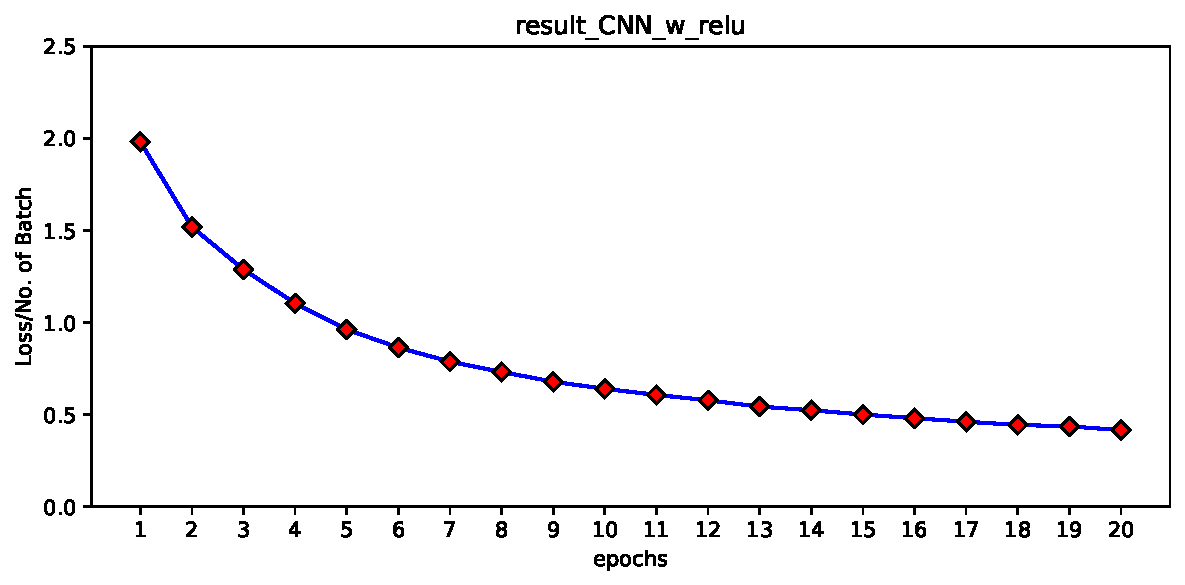
\includegraphics[width=0.45\textwidth]{./results/result_CNN_w_relu.pdf}%
%       \label{fig:cnn_loss}
%    }%
%    % \label{fig:llr_sgd}
%    \hspace{0.5cm}%
%    \subfloat[][CNN Accuracy]
%    {%
%       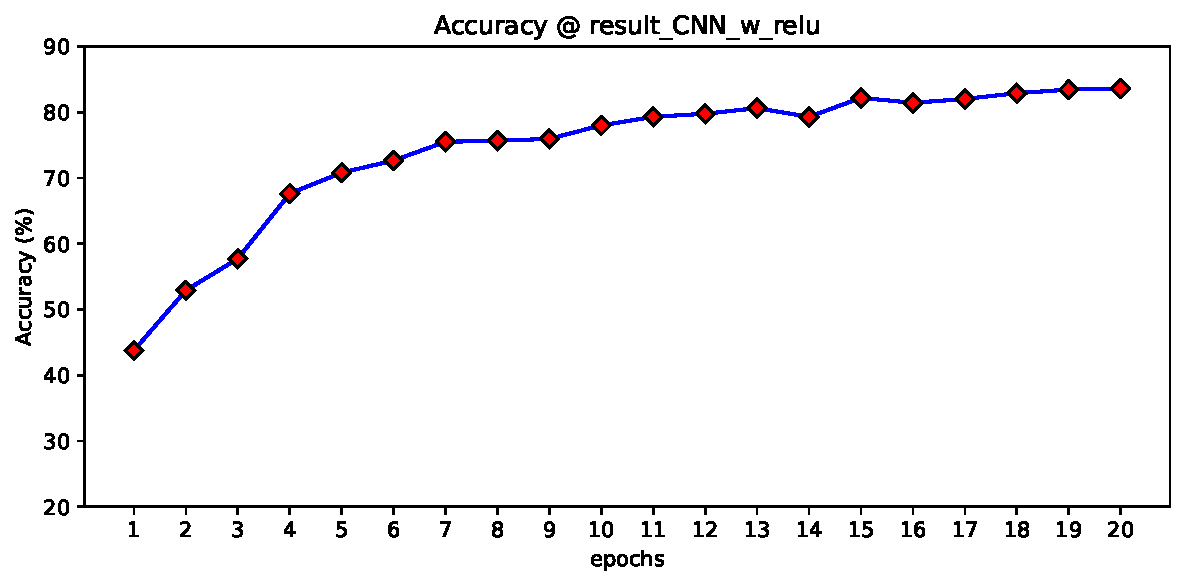
\includegraphics[width=0.45\textwidth]{./results/result_CNN_w_relu_accuracy.pdf}%
%       \label{fig:cnn_acc}
%    }
%    \caption{Convolutional Neural Network training results.}
% \end{figure}
\section*{Bi-LSTM}
The adopted embedding layer is as follows:
the vocabulary size is 18003, and 
embedding dimension is 100.
As for the LSTM structure,
the input size is the same as embedding dimension, which is 100;
the hidden states size is 150, 
and we only deployed 1 layer of LSTM.
No dropout layer is utilized, yet a fully connected layer with 
input size 300, and output size 2 is added to output the final classification results.

\section*{Training Results}
\begin{figure}[!htb]
   \captionsetup[subfigure]{justification=centering}
   \centering
   \subfloat[][LSTM Loss v. Epochs]
   {%
      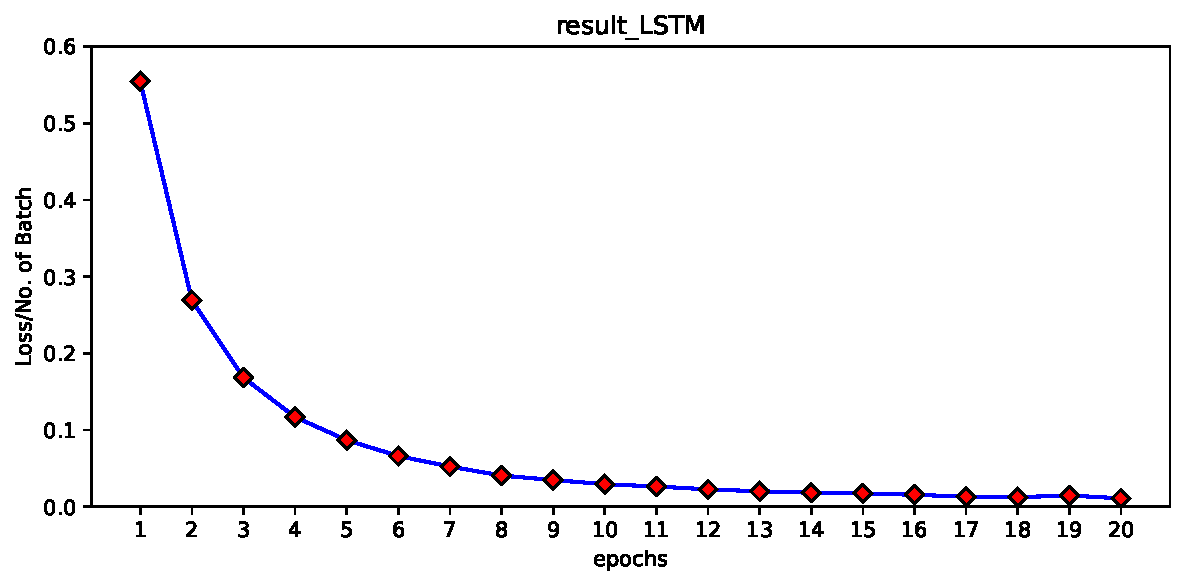
\includegraphics[width=0.45\textwidth]{./results/result_LSTM.pdf}%
      \label{fig:lstm_loss}
   }%
   % \label{fig:llr_sgd}
   \hspace{0.5cm}%
   \subfloat[][LSTM Accuracy]
   {%
      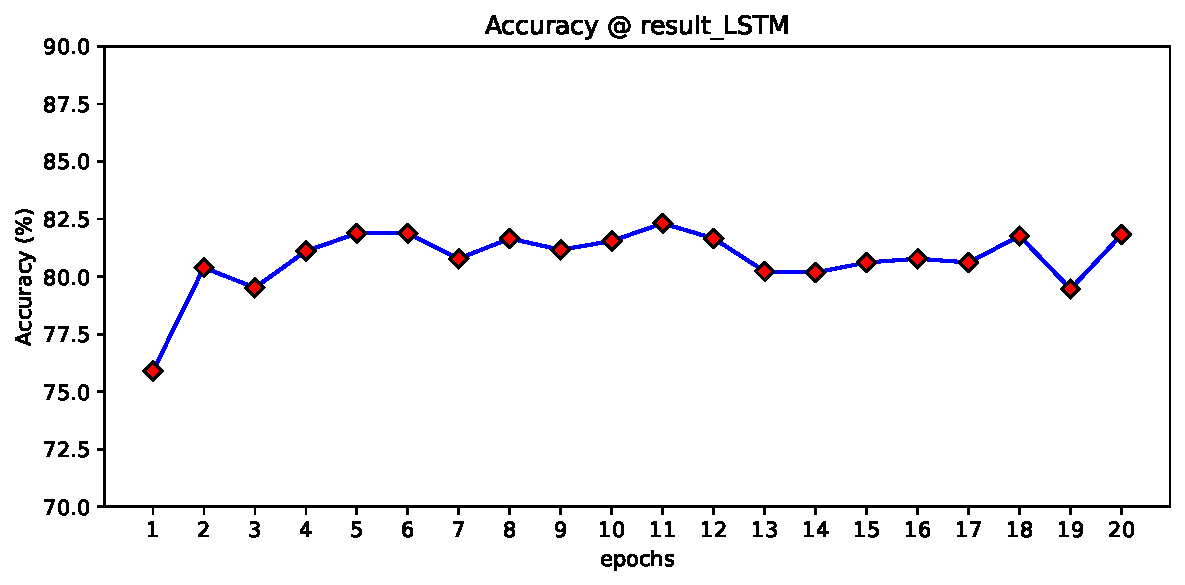
\includegraphics[width=0.45\textwidth]{./results/result_LSTM_accuracy.pdf}%
      \label{fig:lstm_acc}
   }
   \caption{Long Short-Term Memory Network training results.}
\end{figure}
The above shows the final training results. It can be observed that, 
during traning, the loss gradually decreased with the increase of epoch number,
while the accuracy had a trend of improving. 
Nevertheless, it could also be seen that the accuracy experienced a fluctuation after 
reaching around 80\%. 
It could be improved by adding dropout layer, or a better embedding method; or
even improve the entire performance with different framework.


\bibliographystyle{IEEEtran}
% \bibliography{references}

\end{document}

